\newpage
\section{Sprint overview}
\label{sec:sprintOverview}
The following sections summarizes how the project progressed in chronological order. They include the goals the team set for each sprint, and whether these goals were met. The burn down charts and sprint backlog for all of these sprint is to be found in appendix~\ref{sec:sprintbacklog}.

\subsection{Kickoff}
An initial meeting was conducted not long after the team was assigned to this project. Here permanent meeting times, goals and expectations for the project was discussed. All team members agreed to aim for the best grade possible.

\subsection{Sprint 1}
The goals set for this sprint were:\\
$\bullet$\hspace{0.25cm} to have a meeting with the customer,\\
$\bullet$\hspace{0.25cm} get a better grip of what the tasks ahead were,\\
$\bullet$\hspace{0.25cm} research about the task and\\
$\bullet$\hspace{0.25cm} assign all the team members roles.\\\\
After choosing the Scrum approach as the project's framework, a project outline was created, and concepts for the app presented to the customer. The customer was very pleased with the team's ideas, and approved the temporary specification. We also set up the development environment by starting to write documentation in \LaTeX, setting up Android studio and chose Yodiz as project management tool for work distribution and tracking.

\subsection{Sprint 2}
The goals set for this sprint were:\\
$\bullet$\hspace{0.25cm}provide the customer with a working software prototype\\
$\bullet$\hspace{0.25cm}set up the server\\\\
By making this prototype, the team could use it as basis to further develop the requirements specification. Furthermore, a working prototype might help the customer see how the team envisioned the app and its functions. Lastly, work on the server app began to form the foundation a framework of functions that the Android app could use. 

The customer was satisfied with the progress on the prototype, and provided a rich and detailed feedback on how the app should be improved for the next iteration.

\subsection{Sprint 3}
The goals set for this sprint were:\\
$\bullet$\hspace{0.25cm} design prototypes to plan basic functionality\\
$\bullet$\hspace{0.25cm} implement Android GUI for basic functionality\\\\
The team experienced that it was hard to write sections of code without having a GUI design to follow. We therefore decided to design prototypes before starting the implementation, resulting in detailed, digitized prototypes for each part of the app. The team also did some progress on the actual implementation.

During this sprint, some of the team members got sick. This was also a period where other courses at NTNU had big exercise deliveries. The key issue during this sprint was that the effort needed for the other subjects was underestimated. 
%As this is hard to foresee, the team can only but allocate more time to make up for what was lost this sprint.

\subsection{Sprint 4}
The goals set for this sprint were:\\
$\bullet$\hspace{0.25cm} implementing a prototype with functionality from the requirements specification\\
$\bullet$\hspace{0.25cm} complete preliminary report\\
$\bullet$\hspace{0.25cm} peer evaluation\\\\
This sprint had two factors that made it a productive, but also exhausting sprint: Because the previous sprint had not met expectations on completed work, the team compensated for this by working overtime, exceeding the expected working hours by 30 percent. Naturally, the progress was uplifting, but everyone got exhausted from all the extra work. It became apparent that the time required for the tasks made so far had been underestimated. The team agreed it would be better to overestimate and add tasks to the sprint rather than underestimate and not finish the goals set in conjunction with the customer.

\subsection{Sprint 5}
The goals set for this sprint were:\\
$\bullet$\hspace{0.25cm} use prototype as basis to create a software prototype\\
$\bullet$\hspace{0.25cm} implement data synchronization\\
$\bullet$\hspace{0.25cm} replace dummy data with server data\\\\
This sprint, the customer expressed he wanted to become even more involved with the development process by taking part in the sprint start meetings.
% where tasks were estimated, prioritized and allocated resources. 
He also gave us constructive feedback that lead to many major redesigns, particularly in the Android navigation menu. We were made aware of that navigation in what was the main menu at the time could be a challenge. The team used a Kanban board to plan what to focus on in the remaining sprint of the project. This planning process is illustrated in figure~\ref{fig:kanban}.

\begin{figure}[htp]
\centering
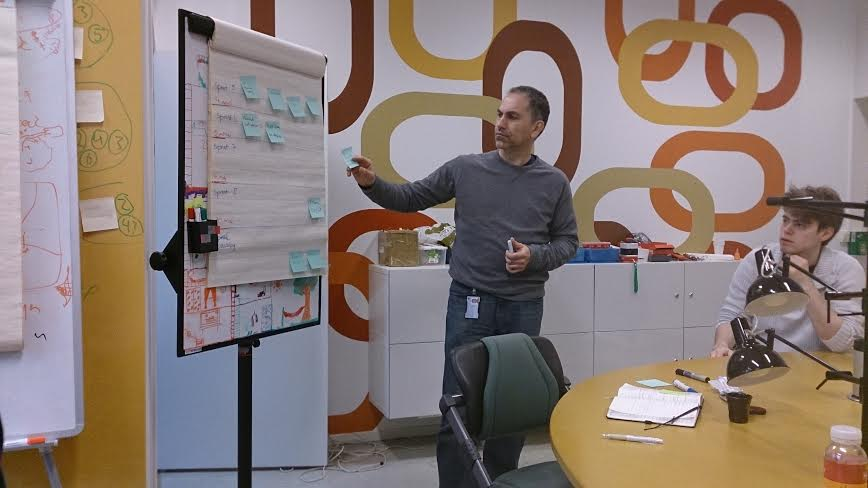
\includegraphics[width=0.75\textwidth, clip, trim=5cm 0cm 0cm 0cm]{ch/devProcess/fig/kanban.jpg}
\caption{Planning process with customer}
\label{fig:kanban}
\end{figure}

\noindent This sprint also had some goals that were not met. Data synchronization was not implemented and all dummy data was not replaced by data from the server based on user credentials. However, most of the apps major functionality was in place, and the team had a pretty clear image of how the finished app would look like and behave.

\subsection{Sprint 6}
The goal set for this sprint was:\\
$\bullet$\hspace{0.25cm} completing all functionality to allow for usability testing, rigorous testing and bug fixing\\\\
Completing the persistence layer was crucial to testing all the apps functionality. All tabs were to be completed at the end of this sprint. The only exception would be particularly tricky problems that required more resources.

After looking at the progress of sprint 6, the team decided it was time to dedicate some extra resources to the documentation. Sprint 5 and 6 had been devoted almost exclusively to development in order to meet deadlines set in cooperation with the customer. Even though generous estimates were made to ensure delivery, the team divided was into two groups as an extra precaution. 

\subsection{Sprint 7}
The goals set for this sprint were:\\
$\bullet$\hspace{0.25cm} to finish development of the app and the server,\\
$\bullet$\hspace{0.25cm} run the test sets in the testing scheme,\\
$\bullet$\hspace{0.25cm} optimize code and fix bugs and\\
$\bullet$\hspace{0.25cm} acquire the customers approval for the finished product.\\\\
The testing revealed performance issues and some major stability issues that had to be resolved before customer approval. Half the team was working intensively on the optimization, while the other half focused on the report. A lot of work, especially in the chapter on further development had to be well under way before the start of sprint 8. After fixing the major issues discovered in testing, the team acquired the customers approval for the finished product on the 16th of May.

\subsection{Sprint 8}
\todo{write sprint 8 summary}